\documentclass{book}
\usepackage{amsmath, amsthm, graphicx, amsfonts, float, bm}
\usepackage[english]{babel}
\graphicspath{ {./images/} }

\usepackage{geometry}
 \geometry{
 a4paper,
 total={170mm,237mm},
 left=20mm,
 top=30mm,
 }
 \usepackage[hidelinks]{hyperref}

\newcommand\eval[2]{\left.#1\right|_{#2}}
\DeclareMathOperator{\sgn}{sgn}
\DeclareMathOperator{\col}{col}
\DeclareMathOperator{\des}{des}
\DeclareMathOperator*{\argmax}{arg\,max}
\DeclareMathOperator*{\argmin}{arg\,min}
\newcommand{\notimplies}{%
  \mathrel{{\ooalign{\hidewidth$\not\phantom{=}$\hidewidth\cr$\implies$}}}}
\newcommand{\R}{\mathbb{R}}
\newcommand{\N}{\mathbb{N}}
\newcommand{\deriv}[1]{\displaystyle\frac{d}{d #1}}
\newcommand{\traj}{(\bar{\mathbf{x}},\bar{\mathbf{u}})}


\theoremstyle{definition}
\newtheorem{definition}{Definition}[section]
\newtheorem{theorem}{Theorem}[section]
\newtheorem{proposition}{Proposition}[section]
\theoremstyle{remark}
\newtheorem*{remark}{Remark}
\theoremstyle{remark}
\newtheorem*{notation}{Notation}
\newtheorem*{result}{Result}
\newtheorem*{observation}{Observation}
\newtheorem*{corollary}{Corollary}

\title{STAC}
\author{Dante Piotto}
\date{November 2022}



% \createtheorem{result}{Result}{SteelBlue3!10}{SteelBlue3!90}{black}

\title{System Theory and Advanced Control}
\author{Dante Piotto}
\date{fall semester 2022}

\begin{document}

\maketitle
\tableofcontents

% \section*{Introduction}
% System Theory and Advanced Control notes, transcribed from notes taken during the lectures held in the fall semester of 2022

\chapter{Dynamic system representation}
\section{system classification}
Dynamic system := system with memory\\
continuous time:
\begin{flalign*}
&    \dot{x}(t) = f(x(t), u(t), t) \qquad x \in \R^n, u \in \R^m\\
&    y(t) = h(x(t), u(t), t) \qquad y \in \R^p
\end{flalign*}
discrete time:
\begin{flalign*}
&    x(t+1) = f(x(t), u(t), t) \qquad x \in \R^n, u \in \R^m\\
&    y(t) = h(x(t), u(t), t) \qquad y \in \R^p
\end{flalign*}
Stationary systems: vector fields $f(\cdot),h(\cdot)$ do not depend on t\\
Linear systems: vector fields $f(\cdot),h(\cdot)$ are linear\\
Autonomous systems: vector fields $f(\cdot),h(\cdot)$ do not depend on $(u(t), t)$\\

\subsection{Linear systems}
\begin{flalign*}
&\left. \begin{array}{r} 
\dot{x}(t)\\[1ex]
{}x(t+1)
\end{array} \right\} 
=A(t)x(t)+B(t)u(t)\\
&y(t)=C(t)x(t) + D(t)u(t)
\end{flalign*}

Stationary linear systems
\begin{align*} 
&\left. \begin{array}{r} 
\dot{x}(t)\\[1ex]
{}x(t+1)
\end{array} \right\} 
=Ax(t)+Bu(t)\\
&y(t)=Cx(t) + Du(t)
\end{align*}

Proper linear systems
\begin{align*} 
&\left. \begin{array}{r} 
\dot{x}(t)\\[1ex]
{}x(t+1)
\end{array} \right\} 
=Ax(t)+Bu(t)\\
&y(t)=Cx(t)
\end{align*}

Autonomous linear systems
\begin{align*} 
&\left. \begin{array}{r} 
\dot{x}(t)\\[1ex]
{}x(t+1)
\end{array} \right\} 
=Ax(t)\\
&y(t)=Cx(t)
\end{align*}

\section{Phase portrait}

\section{Coordinate changes}
A given State Space model implies a coordinate framework in $\R^n$ wrt which the state x is described. A coordinate change for the system is a function $\Phi(\cdot)$, invertible, such that 
\[
z(t)=\Phi(x(t))
\]
z(t) being the system's state in the new coordinate framework.
\subsection{Linear coordinate change}
A linear coordinate change can be expressed by $T:\R^n \to \R^n, \quad z=Tx$ where $T$ is an n x n nonsingular matrix.
\begin{align*} 
&\left. \begin{array}{r} 
\dot{x}(t)\\[1ex]
{}x(t+1)
\end{array} \right\} 
=Ax(t)+Bu(t)\\
&y(t)=Cx(t)+Du(t)
\end{align*}
\begin{align*} 
&\left. \begin{array}{r} 
\dot{z}(t)\\[1ex]
{}z(t+1)
\end{array} \right\} 
=\tilde{A}z(t)+\tilde{B}u(t)\\
&y(t)=\tilde{C}z(t)+\tilde{D}u(t)
\end{align*}
with
\[
\tilde{A}=TAT^{-1} \qquad \tilde{B}=TB \qquad \tilde{C}=CT^{-1} \qquad \tilde{D}=D
\]

\subsection{non-linear coordinate change}
\begin{definition}[Diffeomorphism]
    $\Phi:\R^n\to\R^n$ is said to be a global diffeomorphism if
    \begin{itemize}
        \item it is smooth (differentiable a sufficient number of times)
        \item there exists $\Phi^{-1}: \R^n \to \R^n \quad :\quad \Phi^{-1}(\Phi(x))=x \quad \forall x\in\R^n$
    \end{itemize}
    Local diffeomorphism: same but with $U\subset\R^n$ instead of $\R^n$
\end{definition}
\begin{gather*}
    \dot{x}=f(x)+g(x)u \quad \text{ input-affine system (linear wrt u)}\\ 
    y=h(x)
\end{gather*}
becomes
\begin{gather*}
    \dot{z}=\tilde{f}(z)+\tilde{g}(z)u\\
    y=\tilde{h}(x)
\end{gather*}
where
\begin{gather*}
    \dot{z}=\frac{d\Phi}{dx}\left( f(x)+g(x)u \right) \text{ therefore}\\
    \dot{z}=\eval{\frac{d\Phi}{dx}f(x)}{x=\Phi^{-1}(z)}+\eval{\frac{d\Phi}{dx}g(x)}{x=\Phi^{-1}(z)}u
\end{gather*}
Hence
\begin{gather*}
    \tilde{f}(z):=\eval{\frac{d\Phi}{dx}f(x)}{x=\Phi^{-1}(z)}\\
    \tilde{g}(z):=\eval{\frac{d\Phi}{dx}g(x)}{x=\Phi^{-1}(z)}
    \tilde{h}(z):=h(\Phi^{-1}(z))
\end{gather*}

\begin{result}
    Let $\Phi:\R^n\to\R^n$ be a smooth function, $\bar{x}\in \R^n$ and suppose that $\eval{\frac{d\Phi}{dx}}{\bar{x}}$ is non singular. Then $\Phi(\cdot)$ is a local diffeomorphism at $\bar{x}$. If $\eval{\frac{d\Phi}{dx}}{\bar{x}} \quad \forall \bar{x} \in \R^n$, and $\Phi(\cdot)$ is radially unbounded, then $\Phi(\cdot)$ is a global diffeomorphism
\end{result}

\subsection{Diagonalization of a matrix}
\begin{theorem}

A matrix $A$ is purely diagonalizable by a change of coordinates iff the geometric multiplicity of each eigenvalue is equal to its algebraic multiplicity.

Let $\{\lambda_i,\dots,\lambda_r\}$ be the set of eigenvalues of A, $\{v_{11},\dots,v_{1g_1},{v_{21}},\dots,v_{rg_r}\}$ be the set of associated eigenvectors, and $g_i$ be the associated geometric multiplicity. $A$ can be diagonalized by choosing 
\[
T=\begin{bmatrix}
    v_{11} & \cdots & v_{1g_1} & v_{21} & \cdots & v_{rg_r}
\end{bmatrix}
\]
and we have
\[
\tilde{A}=TAT^{-1}=\begin{pmatrix}
    D_{\lambda_1} & & 0\\
    & \ddots & \\
    0 & & D_{\lambda_r}
\end{pmatrix} \quad \text{with} D_{\lambda_i} = \begin{pmatrix}
    \lambda_i & \cdots & 0\\
    \vdots & \ddots & \vdots\\
    0 & \cdots & \lambda_i
\end{pmatrix} \text{ of dimension } g_i \times g_i
\]
\end{theorem}


\begin{theorem}[Cayley-Hamilton theorem]
Each matrix is solution of its characteristic equation
\[
\varphi(A)=A^n+\alpha_1 A^{n-1}+ \dots + \alpha_{n-1} A + \alpha_nI_n
\]
\end{theorem}

\subsubsection{complex conjugate eigenvalues}
Suppose $\lambda_i = a_i+jb_i$ and $\lambda_{i+1}=a_i-jb_i$, $a_i,b_i \in \R$. Let $v_i=u_i+jw_i, u_i,w_i \in \R^n$ and $v_{i+1}$ be the two linearly independent eigenvectors relative to $\lambda_i, \lambda_{i+1}$. We have that $v_{i+1}=u_i-jw_i$ and that $u_i$ and $w_i$ are linearly independent vectors also linearly independent from all the other eigenvectors.\\
Instead of
\[
T^{-1} = \begin{bmatrix}
    v_1 & v_2 & \cdots & v_i & v_{i+1} & \cdots & v_n
\end{bmatrix}
\]
we can use
\[
T^{-1} = \begin{bmatrix}
    v_1 & v_2 & \cdots & u_i & w_i & \cdots & v_n
\end{bmatrix}
\]
and the resulting matrix is
\[
\begin{pmatrix}
    \lambda_1 & 0 & \cdots & & \cdots & 0 \\
    0 & \lambda_2 & \cdots & &  & \vdots \\
    \vdots & 0 & \ddots & & & \vdots \\
     & \vdots & & \begin{pmatrix}
         a_i & b_i \\
         b_i & a_i \\
     \end{pmatrix} & & \\
      & & & & \ddots & \\
     0 & \cdots & & & \cdots& \lambda_r\\
\end{pmatrix}
\]


\subsection{Jordan form}
\subsubsection{Generalized eigenvectors}
\begin{definition}[generalized eigenvector]
    We say a vector $v \in \R^n$ is a generalized eigenvector (GED\textsubscript{k}) of dimension $k$ linked to $\lambda$ (eigenvalue of $A$) if:
    \begin{gather*}
        (\lambda I -A)^j \neq 0 \quad \forall j \in 0,\dots,k-1 \\
        (\lambda I -A)^kv=0   
    \end{gather*}
\end{definition}
Generalized eigenvectors are linearly independent, and for any $A \in \R^nx\R^n$, there are exactly $n$ generalized eigenvectors. This means that it is always possible to form a base of $\R^n$ of generalized eigenvectors.

Let $\{v_{i1},\dots,v_{i1}^{n_{i1}},\dots,v_{ig_i},\dots,v_{ig_i}^{n_{ig_i}}\}$ be the set of generalized eigenvectors associated to the $i-th$ eigenvalue with geometric multiplicity $g_i$. The Jordan form of the system (with r distinct eigenvalues) is given by a trasformation matrix
\[
T^{-1}=\begin{bmatrix}
    v_{11} & v_{11}^2 & \cdots & v_{1g_1}^{n_1{g_1}} & \cdots & v_{rg_r}^{N_{rg_r}}
    \end{bmatrix}
\]
The system resulting from such transformation has block diagonal form:
\[
\tilde{A} = TAT^{-1} = \begin{pmatrix}
    J_1 & 0 & 0 & \cdots & 0\\
    0 & J_2 & 0 & \cdots & 0\\
    \vdots & \vdots & \vdots &\ddots & \vdots\\
    0 & 0 & 0 & \cdots & J_r
\end{pmatrix}
\]
where the $J_i$ are called Jordan blocks and also have a block diagonal structure
\[
J_i = \begin{pmatrix}
    J_{i1} & 0 & 0 & \cdots & 0\\
    0 & J_{i2} & 0 & \cdots & 0\\
    \vdots & \vdots & \vdots &\ddots & \vdots\\
    0 & 0 & 0 & \cdots & J_{ig_i}
\end{pmatrix}
\]
and the $J_{ik}$ are called mini Jordan blocks
\[
J_{ik} = \begin{pmatrix}
    \lambda_i & 1 & 0 & \cdots & 0\\
    0 & \lambda_i & 1 & \cdots & 0\\
    \vdots & \vdots & \ddots &\ddots & \vdots\\
    0 & 0 & 0 & \cdots & 1\\
    0 & 0 & 0 & \cdots & \lambda_i\\
\end{pmatrix}
\]



\subsection{Schur decomposition}
Given $A \in \R^n \times \R^n$ there always exists a change of variables T such that $\tilde{A}=TAT^{-1}$ is upper(lower) triangular. From a system perspective: given a generic linear system it is possible to see it as the cascade of $n$ scalar subsystems\\
\textbf{read procedure from notes}

\subsection{Brunowsky canonical form}
\begin{definition}[relative degree (SISO case)]
    The triplet (A,B,C) has relative degree r>0 if the following holds:
    \begin{itemize}
        \item $CA^kB=0$ for all $k=0,1,\dots,r-2$
        \item $CA^{r-1}B \neq 0$
    \end{itemize}
\end{definition}
The relative degree $r$ always exists and $r<n$.\\
For continuous time systems, r is the number of times the output needs to be derived in order to see a direct effect on it from the output. \\
we have that \[
rank\begin{pmatrix}
    C\\CA\\\vdots\\CA^{r-1}
\end{pmatrix}=r
\]
i.e., the all the rows are linearly independent
\subsubsection{Brunowsky change of variables}
we choose
\[
T=\begin{pmatrix}
    C\\CA\\ \vdots \\CA^{r-1}\\ \Phi_1 \\ \Phi_2 \\ \vdots \\ \Phi_{n-r}
\end{pmatrix} := \begin{pmatrix}
    T_{\xi} \\ T_{\eta}
\end{pmatrix} \qquad \text{ with the rows of } \Phi_i \text{ chosen so that } T \text{ is not singular}
\]
This leads to the Brunowsky change of variables:
\[
z=\begin{pmatrix}
    \xi \\ \eta
\end{pmatrix} = \begin{pmatrix}
    T_{\xi}x \\ T_{\eta}x = Tx
\end{pmatrix}
\]
This change of variables results in a chain of r integrators, and a "hidden" zero dynamic.
\begin{gather*}
    \xi_1=y \\
    \dot{\xi}_1 = \xi_2 = \dot{y}\\
    \dot{\xi}_2=\xi_3 = \ddot{y}\\
    \vdots \\
    \dot{\xi}_{r-1} = \xi_r\\
    \dot{\xi}_r = CA^{r-1}(Ax+Bu)=CA^rx+CA^{r-1}Bu\\
    \dot{\xi}_r = Q_{\xi} \xi + Q_{\eta}\eta + \Delta u\\
    (Q_{\xi} Q_{\eta}) = CA^rT^{-1} \qquad \Delta = CA^{r-1}B \neq 0
    \\
    \eta = T{\eta} x\\
    \dot{\eta} =T_{\eta}(Ax+Bu)\\
    \dot{\eta} = \Psi_{\xi} \xi + \Psi_{\eta} \eta + T_{\eta}Bu \\ (T_{\eta}B=0 \text{ can always be obtained by construction})
\end{gather*}
If the input is chosen as the state feedback
\[
u(t)=\frac{1}{\Delta}(-Q_{\xi}\xi(t)-Q_{\eta}\eta(t)+v(t))
\]
with $v(t)$ a new residual input, the I-O relation is equivalent to $\frac{1}{s^r}$


\chapter{Stability}
\begin{definition}[$\epsilon-\delta_{\epsilon}$ stability]
    The equilibrium x=0 is stable if $\forall \epsilon>0, \quad \exists \delta_{\epsilon}:\forall ||x(0)||<\delta_{\epsilon}\implies ||x(t)||\leq \epsilon \quad \forall t>0$
\end{definition}
\begin{definition}[asymptotic stability]
    The equilibrium $x=0$ is asymptotically stable if it is stable and there exists a set $\mathcal{A} \supset \{0\}:x(0) \in \mathcal{A}$ implies $\lim_{t \to \infty}x(t)=0$ (attractivity properties). $\mathcal{A}$ is said to be the "Domain of attraction
\end{definition}
\begin{definition}[instability]
    lack of stability
\end{definition}
\begin{theorem}
    A C-T (D-T) linear system is stable iff all the eigenvalues of A have non positive real part (amplitude$\leq 1$) and possible eigenvalues with zero real part (amplitude=1) have a geometric multiplicity equal to the algebraic one. It is asympototically stable iff the eigenvalues of A all have negative real part (amplitude<1)
\end{theorem}
\begin{definition}[positive definite function]
    A function $V:\mathcal{D}\subseteq \R^n \to \R$ is said to be positive definite wrt $\bar{x} \in \mathcal{D}$ if $V(\bar{x})=0$ and $V(x)>0 \forall x \in \mathcal{D} \backslash \{\bar{x}\}$
\end{definition}
\begin{definition}[positive semi-definite function]
    A function $V:\mathcal{D}\subseteq \R^n \to \R$ is said to be positive definite wrt $\bar{x} \in \mathcal{D}$ if $V(\bar{x})=0$ and $V(x)\geq 0 \forall x \in \mathcal{D} \backslash \{\bar{x}\}$
\end{definition}
\begin{definition}[Level set]
    $\Omega_c := \{x\in \R^n : V(x)\leq c\}$
\end{definition}


\begin{theorem}[Direct Lyapunov theorem]
    Let $\bar{x} \in \R^n$ be an equilibrium point for $\dot{x}=f(x)$. Let $V:\mathcal{D}\subseteq \R^n \to \R$ be a positive definite function wrt $\bar{x}\in\mathcal{D}$ and consider the real-valued function $V'(x):\mathcal{D} \to \R$ defined as $V'(x)=\nabla V(x)f(x)$. The following holds:
    \begin{itemize}
        \item if $V'(x)\leq 0 \quad \forall x\in\mathcal{D}$ then $\bar{x}$ is a stable equilibrium point for the system
        \item if $V'(x)< 0 \quad \forall x\in\mathcal{D}$ then $\bar{x}$ is an asympotically stable equilibrium point for the system with a certain domain of attraction $\mathcal{A}$
    \end{itemize}
    For D-T systems the same can be applied but with $V'(x):=V(f(x))-V(x)$
\end{theorem}
\begin{proof}
    Consider a ball of radius $\epsilon$, $\mathcal{B}_{\epsilon}$, contained entirely inside $\mathcal{D}$. This ball contains a level set $\Omega_{\bar{c}}$, which contains a ball of radius $\delta_{\epsilon}$, $\mathcal{B}_{delta_{\epsilon}}$. Since $\forall x \in \mathcal{D},\quad V(x)>0$ and $V'(x)\leq 0$, all trajectories starting inside $\mathcal{B}_{delta_{\epsilon}}$ do not leave $\Omega_{\bar{c}}$, and therefore do not leave $\mathcal{B}_{\epsilon}$.
\end{proof}
\begin{theorem}[Converse Lyapunov theorem]
    let $\bar{x}$ be a stable (asymptotically stable) equilibrium point of $\dot{x}=f(x)$ (with domain of attraction $\mathcal{A}$). Then there exists a differentiable $V:\mathcal{D} \to \R$ that is positive definite wrt $\bar{x}$ (with $\mathcal{D} \supset \mathcal{A}$) and fulfilling $V'(x)\leq 0 (V'(x)<0) \forall x \in \mathcal{D}$. 
\end{theorem}

\begin{theorem}[Direct Lyapunov Theorem (GAS)]
    Let $\bar{x}$ be an equilibrium point for $\dot{x}=f(x)$. Let $V:\R^n\to \R$ be a positive definite function wrt $\bar{x}$ which is radially unbounded ($\|x\|\to\infty\implies V(x)\to\infty$) and consider the real valued function $V'(x):\R^n\to\R$ defined as $V'(x)=\nabla V(x)f(x)$. Then if $V'(x)<0\forall x \in\R^n\backslash\{0\}$, then $\bar{x}$ is GAS.
\end{theorem}

\section{Quadratic forms}
\[V(x)=x^TPx\]
\begin{definition}
    \begin{itemize}
        \item The matrix $P$ is positive semi-definite ($P\geq 0$) if $x^TPx\geq 0 \forall x \in \R^n$
        \item The matrix $P$ is positive definite ($P> 0$) if $x^TPx> 0 \forall x \in \R^n\backslash\{0\}$
        \item The matrix $P$ is negative semi-definite ($P\leq 0$) if $x^TPx\leq 0 \forall x \in \R^n$
        \item The matrix $P$ is negative definite ($P< 0$) if $x^TPx< 0 \forall x \in \R^n\backslash\{0\}$
    \end{itemize}
\end{definition}
Divergence of a quadratic form: $\nabla V(x)=2x^TP$
\begin{observation}
    In quadratic forms the matrix $P$ can be taken symmetric wlog:
    \begin{gather*}
        P_{not symm}=P_{symm}+P_{antisymm} \qquad P_{symm}=\frac{P+P^T}{2} \quad P_{antisymm}=\frac{P-P^T}{2}\\
        \implies x^TPx=x^T(P_{symm}+P_{antisymm})x=x^TP_{symm}x+x^TP_{antisymm}x\\
        (x^TP_{symm}x)^T=x^TP_{symm}^Tx=x^TP_{symm}x\\
        (x^TP_{antisymm}x)^T=x^TP_{antisymm}^Tx=-x^TP_{antisymm}x \implies \\ 
        \implies x^TP_{antisymm}x=0 \text{ because } x^TP_{antisymm}x \text{ is a scalar}
    \end{gather*}
\end{observation}

\begin{result}
    A matrix $P$ is positive definite iff all its leading principal minors are positive.
\end{result}
Properties of symmetric positive definite matrices $P$:\begin{itemize}
    \item $P$ is diagonalizable $(a_i=g_i)$
    \item The eigenvalues $\lambda_i$ and eigenvectors $v_i$ are real, $i=1,\dots,n$
    \item $\lambda_i>0, i=1,\dots,n$, and for each pair $(v_i,v_j)$ of eigenvectors $<v_i,v_j>=0$ (orthogonal)
\end{itemize}
Geometry of $\Omega_c=\{x\in\R^n \quad : \quad x^TPx\leq c\}$:

$\Omega_c$ are ellipsoids with their principal axes direct as the eigenvectors of $P$ and amplitude proportional to the relative eigenvalues.

\section{Linear systems}
\begin{flalign*}
    &\left. \begin{array}{r} 
        \dot{x}(t)\\[1ex]
        {}x(t+1)
        \end{array} \right\} 
        =Ax(t) \qquad x(0)=x_0 \hfill V(x)=x^TPx
\end{flalign*}
\begin{theorem}
    \begin{enumerate}
        \item The system is Hurwitz(Schur) iff there exists $P=P^T>0$ and $Q=Q^T>0$ solution of the Lyapunov matrix equation:\[
            PA+A^TP=-Q \quad \text{ (C-T)} \qquad \qquad A^TPA-P=-Q \quad \text{ (D-T)}\]
        \item If there exists a solution $(P,Q)$ then there exists an infinite number of other solutions, one for each $Q=Q^T>0$. That is, $Q$ is arbitrary.
        \item If the Lyapunov matrix equations are fulfilled with $Q=Q^T\geq 0$ then the system is stable
    \end{enumerate}
\end{theorem}
\begin{proof}(1)
    $\implies$: pick 
    \[
        P=\int_0^\infty e^{A^Ts}Qe^{As}\,ds\
    \]
    with $Q$ generic. The integrand is a sum of exponential vanishing terms, and therefore the integral exists. We have that
    \begin{gather*}
        PA+A^TP=\int_0^\infty e^{A^Ts}Qe^{As}A\,ds\ + \int_0^\infty A^Te^{A^Ts}Qe^{As}\,ds\ =\int_0^\infty \frac{d}{ds} e^{A^Ts}Qe^{As}\,ds\ = \eval{e^{A^Ts}Qe^{As}}{0}^\infty = -Q
    \end{gather*}
    If $Q$ is symmetric, i.e. $Q=Q^T$, then
    \[
        P^T= \left[ \int_0^\infty e^{A^Ts}Qe^{As}\,ds\ \right]^T=\int_0^\infty\left[ e^{A^Ts}Qe^{As} \right]^T\,ds\ = \int_0^\infty e^{A^Ts}Qe^{As}\,ds\ =P
    \]
    Which proves $P$ is also symmetric. To prove it is positive definite, we can consider that if $Q=Q^T>0$
    \[
        x^TPx=x^T\int_0^\infty e^{A^Ts}Qe^{As}\,ds\ x >0 \forall s 
    \]
    because $A$ is Hurwitz.\\
    $\impliedby$: pick $V(x)=x^TPx$. We have
    \[
        V'(x)=<\nabla V(x),f(x)>=2x^TPAx = x^TPAx+x^TPAx=x^TPAx+x^TA^TPx
    \]
    therefore
    \[
        V'(x)=x^T(PA+A^TP)x=-x^TQx
    \]
    if there exists $Q=Q^T>0$ then due to the Direct Lyapunov Theorem the system is GAS.
\end{proof}

\begin{theorem}[indirect Lyapunov theorem]
    \begin{enumerate}
        \item Suppose that there exists a $P=P^T>0$ and $Q=Q^T>0$ solution of the Lyapunov matrix equation. Then $\bar{x}$ is LAS for $\dot{x}=f(x)$ with a certain domain of attraction ($V=(x-\bar{x})^TP(x-\bar{x})$ is a possible candidate Lyapunov function)
        \item Suppose that $A$ has at least one eigenvalue with positive real part. Then $\bar{x}$ is unstable for $\dot{x}=f(x)$ 
    \end{enumerate}
\end{theorem}
\begin{proof}[(1)]
    Let's assume wlog $\bar{x}=0$.
    \[
        \dot{x}=Ax+g_h(x)
    \]
    where $g_h(x)$ represents the higher order terms of $f(x)$. Picking $V(x)=x^TPx$ we have:
    \[
        V'(x)=2x^TP(Ax+g_h(x))=x^T(PA+A^TP)x+2x^TPg_h(x)=-x^TQx+2x^TPg_h(x)
    \]
    The first term on the right-hand side is negative definite, while the second term is in general indefinite. The function $g_h(x)$ satisfies
    \[
        \frac{\|g_h(x)\|}{\|x\|}\to 0 \text{ as } \|x\|\to 0 
    \]
    Therefore, for any $\gamma>0$ there exists $r_\gamma>0$ such that
    \[
        \|g_h(x)\|<\gamma\|x\|, \quad \forall \|x\|<r_\gamma
    \]
    Hence,
    \[
        V'(x)<-x^TQx+2\gamma \|P\|\|x\|^2, \quad \forall \|x\|<r_\gamma
    \]
    but
    \[
        x^TQx\geq \lambda_{min}(Q)\|x\|^2
    \]
    where $\lambda_{min}(\cdot)$ denotes the minimum eigenvalue of a matrix. Note that $\lambda_{min}(Q)$ is real and positive since $Q$ is symmetric and positive definite. Thus
    \[
        V'(x)<-\left[ \lambda_{min}(Q)-2\gamma\|P\| \right]\|x\|^2, \quad \forall \|x\|<r_\gamma
    \]
    Choosing $\gamma<\lambda_{min}(Q)/2\|P\|$ ensures that $V'(x)$ is negative definite. By the Lyapunov direct theorem, we conclude that the origin is asympotically stable.
\end{proof}

\begin{observation}
    A conservative estimate for the domain of attraction is the largest level set contained in the ball of radius $\lambda_{min}(Q)/4\|P\|$\\
    The theorem is not conclusive when $A$ has eigenvaues on the imaginary axis. In this case the system is said to be non hyperbolic at $\bar{x}$. In the non-hyperbolic case the equilibrium could be either stable, asymptotically stable or unstable for the non linear dynamics. The high-order terms play a role in determining the stability properties of the system.
\end{observation}

\section{Krasovski-La Salle Criterion}


\begin{definition}[invariant set]
    A set $M$ is invariant for $\dot{x}=f(x)$ if, having denoted by $x(t,x_0)$ the trajectory at time $t$ with initial condition $x_0$ at time $t=0$, then
    \[
        x_0\in M \implies x(t,x_0)\in M \forall t \in \R
    \]    
\end{definition}

\begin{theorem}[Krasovski-La Salle Criterion]
    Let $V:\mathcal{D}\subseteq \R^n\to\R$ be a positive definite function relative to $\bar{x}$, an equilibrium point of the system $\dot{x}=f(x)$. Suppose that $V'(x)\leq 0 \quad \forall x\in\mathcal{D}'\subseteq \mathcal{D}$. Let $E\subseteq \mathcal{D}'$ be a set where $V'(x)=0$ and let $M$ be the largest set contained in $E$ which is invariant for the trajectories of the system. Then:
    \begin{itemize}
        \item the equilibrium $\bar{x}$ is stable
        \item the set $M$ is attractive for the trajectories of the system, namely \[\lim_{t\to\infty}dist(x(t),M)=0\]
    \end{itemize}
\end{theorem}
\begin{corollary}
    if $M=\bar{x}$ then the equilibrium point is asympototically stable.
\end{corollary}

\section{Systms with inputs and outputs}
\begin{definition}[Input to State Stability (ISS)]
    A system $\dot{x}=f(x,u)$ fulfilling $f(0,0)=0$ is ISS with respect to $\bar{x}=0$ if there exists a positive definite real valued function $V:\mathcal{D}\to \R$ (ISS Lyapunov function) and a strictly increasing function $\chi:\R\to\R$ fulfilling 
    \[
        \|x\|\geq\chi(\|u\|) \quad \implies \quad V'(x,u)= \nabla V(x)f(x,u)<0
    \]
\end{definition}

\begin{definition}[passivity]
    A system with an input and output ($\dot{x}=f(x,u)$, $y=h(x)$) is said to be passive if there exists a positive definite real valued function $V:\mathcal{D}\to\R$ (storage function) fulfilling
    \[
        \dot{V}(x(t))=V'(x,u)=\nabla V(x)f(x,u)\leq u^Ty
    \]
\end{definition}
Interpretation: the energy stored in the system in a time interval should be $\leq$ than the energy supplied to it.






\chapter{Geometry of trajectories}
eigenvalues go \textbf{BRRR}














\chapter{Reachability and controllability}
\section{Reachability}
\begin{definition}[Reachability]
    Set of reachable states  at time $t_1$:
    \[
        \mathcal{R}^+(t_1)=\{x\in \R^n : x = \Psi(t_1)u([0,t_1)) \text{ for some }u([0,t_1)) \in \R^m\}
        \]
    Reachable set:
    \[
        \mathcal{R}^+:=\mathcal{R}^+(\infty)
    \]
\end{definition}
\begin{theorem}
    \(\mathcal{R}^+=Im(R) \qquad R=\begin{bmatrix}
        B & AB & A^2B & \cdots & A^{n-1}B
    \end{bmatrix}\)
\end{theorem}
\begin{proof}[D-T case]
    we assume \(x(0)=0\). We have that the state at time $t$ can be expressed by
    \begin{gather*}x(t)=A^tx_0+\sum_{i=0}^{t-1} A^{t-1-i}Bu(i)\\
    x(1)=Bu(0)\\
    x(2)=ABu(0)+Bu(1)\\
    x(3)=A^2Bu(0)+ABu(1)+Bu(2)\\
    x(t)=\begin{bmatrix}
        B & AB & \cdots & A^{t-1}B
    \end{bmatrix}\begin{bmatrix}
        u(t-1)\\\vdots\\u(0)
    \end{bmatrix} = R_tu_0^{t-1}
    \end{gather*}
    we need to prove that \(ImR_t=ImR_n \forall t \in \N:t\geq n\):
    \(R_t=\begin{bmatrix}
        B & AB & \cdots & A^{n-1} | A^nB & A^{n+1} & \cdots
    \end{bmatrix}\). By the Cayley Hamilton theorem we have that
    \begin{gather*}
    \varphi_A(A)=A^n+\alpha_1A^{n-1}+\dots+\alpha_nI_n=0 \implies A^nB+\alpha_1A^{n-1}B+\dots+\alpha_nB=0\\
    \implies A^nB \text{ is L.D from } \{B,AB,\dots,A^{n-1}B\}
    \end{gather*}
    This can be extended to $A^{n+1}$ by premultiplying by A.\\
    From this proof we have the added observation that for D-T systems if a state is reachable it is reachable in at most $n$ steps
\end{proof}

\begin{theorem}[PBH Test]
    The pair $(A,B)$ is completely reachable iff $rank\begin{bmatrix}
        \lambda I-A & B
    \end{bmatrix}=n \quad \forall \lambda \in \sigma(A)$
\end{theorem}
\begin{proof}
    get it done hints in paper notes
\end{proof}

\section{Computing the input}

\subsection{D-T case}
Since \(x(t)=R_tu_0^{t-1}\):\\
case \(\mathcal{R}^+=\R^n, t\geq n\)
\[
\bar{x}=R_tu_0{t-1} \qquad u_0{t-1}=R^T_t(R_tR^T_t)=^{-1}\bar{x}
\]
where $R_t$ is a fat full row rank matrix\\
general case (\(t<n, \mathcal{R}\subset \R^n\)). The target state, in order to be reached, must fulfil \(\bar{x} \in ImR_t\)
\[
\bar{x}=R_tu_0^{t-1} \qquad u_0^{t-1}={R}_t^{\dagger} \bar{x}
\]
The Moore-Penrose pseudoinverse, if the matrix is (right) invertible, boils down to the canonical (right) inverse. Otherwise, it provides a unique solution to \(\bar{x}=R_tu_0{t-1}\) if it has one, or if \(\bar{x}\notin ImR_t\) it provides the closest solution in the Euclidean sense.
\[
||\bar{x}-R_tR_t^{\dagger}\bar{x}||\leq ||\bar{x}-R_tu_0^t|| \text{ with } u_0^t \text{ generic input sequence}
\]

\subsection{C-T case}
We introduce the reachablity/controllability Gramian at time t:
\[
W(t)=\int_0^te^{A(t-s)}BB^Te^{A^{T(t-s)}}\,ds\
\]
\begin{result}
    The Gramian is non singular for each $t>0$ iff $\mathcal{R}^+=\R^n$
\end{result}
let's pick \(u(s)=\left[e^{A(t-s)}B\right]^TV(s)\) with $V(s)$ generic for now. From Lagrange we have
\[
x(t)=\int_0^t e^{A(t-s)}Bu(s)\,ds\ =\int_0^t e^{A(t-s)}B B^Te^{A^T(t-s)}V(s)\,ds\
\]
where \(e^{A(t-s)}B B^Te^{A^T(t-s)}\) is an $nxn$ supersingular square matrix. If $V(s)$ is constant, we have
\[
\bar{x}=x(t)=W(t)V
\]
and we can pick \(V=W^{-1}(t)\bar{x}\), resulting in:
\[
u(s)=B^Te^{A^T(t-s)}W^{-1}(t)\bar{x} \qquad s\in [0,t)
\]
if $x_0\neq 0$, because of linearity the problem can be cast as the problem of steering the state of the system from the origin to the final target in a  predetermined interval:
\[
    x(t)=e^{At}x_0+\int_0^t e^{A(t-s)}Bu(s)\,ds\ \implies u(s)=B^Te^{A^T(t-s)}W^{-1}(t)(\bar{x}-e^{At}x_0) \qquad  s\in [0,t)
\]
\section{Controllability}

\begin{definition}[Controllability]
    Set of controllable states  at time $t_1$: \(\mathcal{R}^-(t_1)=\{x\in \R^n : x = \Phi(t_1)x+\Psi(t_1)u([0,t_1)) \text{ for some }u([0,t_1)) \in \R^m\}\)\\
    Controllable set: \(\mathcal{R}^-:=\mathcal{R}^-(\infty)\)
\end{definition}

\begin{theorem}
    \( \mathcal{R}^+ \supseteq \mathcal{R}^- \) in general. \(\mathcal{R}^+ = \mathcal{R}^-\) if the system is reversible
\end{theorem}

\section{Controllability and state feedback}
Controllability properties are invariant to change of coordinates, and are therefore properties of the system:\\
\begin{gather*}
    (\tilde{A}, \tilde{B})=(TAT^{-1},TB)\\
    \tilde{R}=\begin{bmatrix}
        \tilde{B} & \tilde{A}\tilde{B} & \cdots & \tilde{A}^{n-1}\tilde{B}
    \end{bmatrix}=TR \implies ImR=Im\tilde{R}
\end{gather*}

\begin{theorem}
    $(A,B)$ completely controllable $\implies (A+BK,B)$ completely controllable $\forall K$
\end{theorem}
\begin{proof}
    We can apply the PBH test. Assuming
    \begin{gather*}
        A=\begin{pmatrix}
            a_{11} & a_{12}& \cdots & a_{1n}\\
            a_{21} & a_{22}& \cdots & a_{2n}\\
            \vdots & \vdots& \ddots & \vdots\\
            a_{n1} & a_{n2}& \cdots & a_{nn}\\
        \end{pmatrix}\qquad B=\begin{pmatrix}
            b_1 \\ b_2 \\ \vdots \\ b_n
        \end{pmatrix} \qquad K=\begin{pmatrix}
            k_1 & k_2 & \cdots & k_n
        \end{pmatrix}
    \end{gather*}
    we have that
    \begin{gather*}
        \begin{bmatrix}
            \lambda I -(A+BK) & B
        \end{bmatrix}=\begin{pmatrix}
            \lambda-a_{11}-b_1k_1 & -a_{12}-b_1k_2& \cdots & -a_{1n}-b_1k_n & b_1\\
            -a_{21}-b_2k_1 & \lambda-a_{22}-b_2k_2& \cdots & -a_{2n}-b_1k_n & b_2\\
            \vdots & \vdots & \ddots & \vdots & \vdots\\
            -a_{n1}-b_nk_1 & -a_{n2}-b_nk_2& \cdots & \lambda-a_{nn}-b_nk_n & b_n\\
        \end{pmatrix}
    \end{gather*}
    we can apply the following column substitutions without altering the rank of the matrix:
    \begin{gather*}
        c_i\rightarrow c_i+c_{n-1}k_i \qquad i=1,\dots,n
    \end{gather*}
    and we obtain the following matrix
    \begin{gather*}
        \begin{pmatrix}
            \lambda-a_{11} & -a_{12}& \cdots & -a_{1n} & b_1\\
            -a_{21} & \lambda-a_{22}& \cdots & -a_{2n} & b_2\\
            \vdots & \vdots & \ddots & \vdots & \vdots\\
            -a_{n1} & -a_{n2}& \cdots & \lambda-a_{nn} & b_n\\
        \end{pmatrix}=\begin{bmatrix}
            \lambda I -A & B
        \end{bmatrix}
    \end{gather*}
    Therefore, because rank \( \begin{bmatrix}
        \lambda I -A & B
    \end{bmatrix}=n \) due to it being fully controllable, we conclude that \((A+BK,B)\) is fully controllable $\forall K$
\end{proof}
\subsection{controllablilty canonical form}
\begin{gather*}
A_c=\begin{pmatrix}
    0 & 1 & 0 & \cdots & 0 \\
    0 & 0  & 1 & \cdots & 0 \\
    \vdots & \vdots & \vdots & \ddots & 1\\
    -\alpha_n & -\alpha_{n-1} & -\alpha_{n-2}& \cdots & -\alpha_1
\end{pmatrix} \qquad B_c=\begin{pmatrix}
    0 \\ \vdots \\ 0 \\1
\end{pmatrix} \\ \varphi_A(\lambda)=det(\lambda I-A)=\lambda^n+\alpha_1\lambda^{n-1}+\dots+\alpha_{n-1}\lambda +\alpha_n
\end{gather*}

\begin{theorem}
    $m=1$\\
    A pair $(A,B)$ is similar to $(A_c,B_c)$ $\iff$ the system is completely controllable
    \begin{gather*}
        T=T_c:=R_cR^{-1}\\
        R_c=\begin{bmatrix}
            B_c & A_cB_c & \cdots & A_c^{n-1}B_c
            \end{bmatrix}
    \end{gather*}

\end{theorem}

\begin{theorem}[Eigenvalues assignment theorem]
    A pair $(A,B)$ is completely controllable $\iff$ for all \(\{\lambda_1^{\star},\dots,\lambda_n^{\star}\}\) (set of desired eigenvalues) there exists a $K$ such that $\sigma(A+BK)=\{\lambda_1^{\star},\dots,\lambda_n^{\star}\}$
\end{theorem}
\begin{proof}[($\implies$)]
    let $(\alpha_1^{\star},\dots,\alpha_n^{\star})$ be s.t. $\{\lambda_1^{\star},\dots,\lambda_n^{\star}\}$ are roots of $\lambda^n+\alpha_1^{\star}\lambda^{n-1}+\dots+\alpha_{n-1}^{\star}\lambda +\alpha_n^{\star}=0$ \\
    since $(A,B)$ is completely controllable it can be cast into controllability canonical form through a $T_c$. Considering a generic $K_c$ we have that
    \[
    A_c+B_cK_c=\begin{pmatrix}
    0 & 1 & 0 & \cdots & 0 \\
    0 & 0  & 1 & \cdots & 0 \\
    \vdots & \vdots & \vdots & \ddots & 1\\
    -\alpha_n & -\alpha_{n-1} & -\alpha_{n-2}& \cdots & -\alpha_1
\end{pmatrix} +\begin{pmatrix}
    0 \\ \vdots \\ 0 \\1
\end{pmatrix} \begin{pmatrix}
    K_{c_1} & \cdots & K_{c_n}
\end{pmatrix}
    \]
    we can pick
        \[
    K_c=(\alpha_n-\alpha_n^{\star},\dots,\alpha_1-\alpha_1^{\star})
    \]
    resulting in the desired eigenvalues. The matrix K is found as follows:
    \begin{gather*}
        z=T_cx \\
        u=K_cz+v \\
        \dot{z}=(A_c+B_cK_c)u+B_cv \\
        u=K_cT_cx \\
        K=K_cT_c \\
    \end{gather*}
    
\end{proof}

\section{Kalman Decomposition}
\begin{definition}[stabilizable system]
    A system $(A,B)$ is stabilizable if there exists $K$ s.t. $(A+BK)$ is Hurwitz(Schur)
\end{definition}

Suppose that $(A,B)$ is not completely controllable, namely rank$R=n_r<n$\\
Let $\mathcal{R}^+_{\perp}$ be the orthogonal complement of $\mathcal{R}^+$. It turns out that dim$\mathcal{R}^+_{\perp}=n-n_r$ \\
Let $\{v_1,\dots,v_{n_r}\}$ be a base of $\mathcal{R}^+$ and let $\{v_{n_r+1},\dots,v_n\}$ be a base of $\mathcal{R}^+_{\perp}$. The two sets of vectors are all linearly independent\\
Consider the change of variables \begin{gather*}
    T_K^{-1}=\begin{bmatrix}
    v_1 &  \cdots & v_{n_r} & v_{n_r+1} & \cdots & v_n
\end{bmatrix}\\
z=T_Kx=\begin{pmatrix}
    z_r \\ z_{n_r}
\end{pmatrix} \qquad x=T_K^{-1}z
\end{gather*}

it turns out that $x\in \mathcal{R}^+ \implies z= \begin{pmatrix}
    \star \\ 0
\end{pmatrix} \qquad x\in\mathcal{R}^+_{\perp} \implies z= \begin{pmatrix}
    0 \\ \star
\end{pmatrix}$ 
\begin{result}
\[
    \tilde{A}_K=T_KAT_K^{-1}=\begin{pmatrix}
        \tilde{A}_R & \tilde{A}_J\\
        0 & \tilde{A}_{NR}
    \end{pmatrix} \qquad \qquad \tilde{B}_K=T_KB=\begin{pmatrix}
        \tilde{B}_R \\ 0
    \end{pmatrix} \qquad \qquad (\tilde{A}_R,\tilde{B}_R) \text{ completely reachable}
\]
\end{result}
with  $\tilde{A}_R$ $n_r\times n_r$ and $\tilde{A}_{NR}$ $n-n_r \times n-n_r$.\\
\begin{itemize}
    \item The set $\mathcal{R}^+$ is forward invariant for the system dynamics. The "internal dynamics" are completely reachable/controllable
    \item if $\tilde{A}_{NR}$ is Hurwitz then trajectories starting outside $\mathcal{R}^+$ asymptotically converge to it
\end{itemize}

\begin{theorem}
    $(A,B)$ is stabilizable $\iff$ $\tilde{A}_{NR}$ is Hurwitz(Schur)
\end{theorem}
\begin{proof}[$\impliedby$]
    Let $(A,B)$ be generic, with $\mathcal{R}^+\subset \R^n$. By Kalman,
    \[
    \exists T_K:T_KAT_K^{-1}=\tilde{A}_K=\begin{pmatrix}
        \tilde{A}_R & \tilde{A}_J\\
        0 & \tilde{A}_{NR}
    \end{pmatrix} \qquad T_KB=\tilde{B}_K= \begin{pmatrix}
        \tilde{B}_R \\ 0
    \end{pmatrix}
    \]
    In the Kalman Coordinates, we can design a $K_K=\begin{bmatrix}
        K_{K_R} & K_{K_{NR}}
    \end{bmatrix}$ such that $\tilde{A}_R+\tilde{B}_RK_{K_R}$ is Hurwitz.:
    \[
        \tilde{A}_K+\tilde{B}_KK_{K}=\begin{pmatrix}
            \tilde{A}_R+\tilde{B}_RK_{K_R} & \tilde{A}_J+\tilde{B}_RK_{K_R}\\
            0 & \tilde{A}_{NR}
        \end{pmatrix} \implies \sigma(\tilde{A}_K+\tilde{B}_KK_{K})=\sigma(\tilde{A}_R+\tilde{B}_RK_{K_R})\cup \sigma(\tilde{A}_{NR})
    \]
    The eigenvalues of $(\tilde{A}_R,\tilde{B}_R$ are completely assignable because it is a completely controllable pair by construction, and the eigenvalues of $\tilde{A}_{NR}$ are stable by definition. We can thus pick
    \[
    K_K=\begin{bmatrix}
        K-{K_R} & \star
    \end{bmatrix}
    \]
    and because
    \[
    z=T_Kx \implies u=K_KT_Kx+v
    \]
    we have that
    \[
    K=K_KT_K
    \]
\end{proof}



\section{controllability of a cascade}

\begin{result}
    The cascade is controllable $\iff$ the subsystems are controllable and the zeros of the first subsystem do not resonate with the poles of the second subsystem, namely
    \[
    rank\begin{pmatrix}
        A-\lambda I & B\\
        C & 0
    \end{pmatrix}=n+1 \qquad \forall \lambda \in \sigma(F)
    \]
\end{result}



\chapter{Observability and reconstructability}
\section{Observability}
\begin{definition}[Set of unobservable states]
    Set of unobservable states in $[0,t_1)$
    \[
        \mathcal{E}^+_{NO}(t_1) = \{x\in \R^n : C\Phi(t)x=0 \forall t \in [0,t_1)
    \]
    Unobservable set: $\mathcal{E}^+_{NO}:=\mathcal{E}^+_{NO}(\infty)$
\end{definition}
\begin{result}
    the unobservable set $\mathcal{E}^+_{NO}$ is a subspace of $\R^n$
\end{result}

\begin{theorem}
    \[
    \mathcal{E}^+_{NO} = Ker(O) \qquad O:=\begin{bmatrix}
        C\\CA\\CA^2\\\vdots\\CA^{n-1}
    \end{bmatrix}
    \]
    O is called the Observability matrix
\end{theorem}
\begin{proof}
    \begin{align*}
        y(0)=Cx_0\\
        y(1)=Cx(1)=CAx_0\\
        y(2)=Cx(2)=CA^2x_0\\
        y(t)=CA^tx_0\\
        \implies y_0^{t-1}=\begin{bmatrix}
            y(0)\\y(1)\\\vdots\\y(t-1)
        \end{bmatrix}=\begin{bmatrix}
            C\\CA\\\vdots\\CA^{t-1}
        \end{bmatrix}x_0=O_tx_0
    \end{align*}
    The set of $x_0$ s.t. $y(t)=0 \forall t<n$ is $KerO_n=\mathcal{E}^+_{NO}(n)$\\
    We need to prove that $KerO_t=KerO_n \forall t \in \N : t>n$\\
    Due to Cayley-Hamilton $\varphi_A(A)=A^n+\alpha_1A^{n-1}+\dots+\alpha_nI_n=0$, and therefore, premultiplying by C we have
    \begin{flalign*}
        CA^m=\alpha_1CA^{n-1}+\dots+\alpha_nC \quad \implies \quad CA^n \text{ is L.D. from } \{C,CA,\dots,CA^{n-1}\} \\ \implies rank(O_{n+1})=rank(O) \implies ker(O_{n+1}=ker(O). \\ \text{ This can be extended to }O_{n+i} \text{ by premultiplying by } CA^{i}
    \end{flalign*}
\end{proof}
\begin{definition}[Observability]
    observable set: $\mathcal{E}^+=[\mathcal{E}^+_{NO}$
\end{definition}
\begin{observation}
    $KerM=(ImM^T)_{\perp}$ with M a generic matrix. Hence:
    \[
    \mathcal{E}^+=Im[O^T]  \qquad O^T:=\begin{bmatrix}
        C^T & A^TC^T & (A^T)^2C^T & \cdots & (A^T)^{n-1}C^T
    \end{bmatrix}
    \]
\end{observation}



\begin{theorem}[PBH test]
    the pair $(A,C)$ is completely observable $\iff$ 
    \[
    rank\begin{bmatrix}
        \lambda I- A \\ C
    \end{bmatrix}=n \qquad \forall \lambda (\in \sigma(A))
    \]
\end{theorem}
\begin{proof}
    get it done (lazy cunt)
\end{proof}

\section{Reconstructing the state from the output}
\subsection{D-T case}
since $y_0^{t-1}=O_tx(0)$:
case $\mathcal{E}^+=\R^n, t\geq n$:
\[
    y_0^{t-1}=O_tx(0) \qquad x(0)=(O_t^TO_t)^{-1}O_t^Ty_0^{t-1}
\]
where $O_t$ is a tall full column rank matrix

General case ($t<n, \mathcal{E}^+\subset \R^n$): the initial state $x(0)$ must fulfil $y_0^{t-1}\in ImO_t$. In these cases the equaton $y_0^{t-1}=O_tx(0)$ can be solved for $x(0)$:
\[
x(0)=O_t^{\dagger}y_0^{t-1}
\]
If an input is present we can still solve the problem by defining a generalised output:
\[
    y(t)-\sum_{i=0}^{t-1}CA^{t-i-1}Bu(i)=\bar{y}(t)=CA^tx(0)
\]
\subsection{C-T case}
from Lagrange:
\[
y(t)=Ce^{At}x_0 \implies \int_0^te^{A^Ts}C^Ty(s)\,ds\ = \int_0^te^{A^Ts}C^TCe^{As}x_0\,ds\
\]
where $e^{A^Tt}C^TCe^{At}$ is an $n \times n$ supersingular matrix.
We define the observability Gramian as such:
\[
V(t)=\int_0^te^{A^Ts}C^TCe^{As}\,ds\
\]
\begin{result}
    The Gramian is non singular for each $t>0$ iff $\mathcal{E}^+=\R^n$
\end{result}
if the Gramian is non singular we can compute the input as follows:
\begin{align*}
    V(t)x_0=\int_0^te^{A^Ts}C^Ty(s)\,ds\ \\
    \implies x_0=V^{-1}(t)\int_0^te^{A^Ts}C^Ty(s)\,ds\
\end{align*}
If there is an input present we can define a generalized output:
\begin{gather*}
    Ce^{At}x_0=y(t) - \int_0^t e^{A(t-s)}Bu(s)\,ds\ \\
    \bar{y}(t):=y(t)-\int_0^t e^{A(t-s)}Bu(s)\,ds\ \\
    \implies x(0)=V^{-1}(t)\int_0^t {e^{A^Ts}C^T \left[ y(s) - \int_0^s e^{A(s-s')}Bu(s') \, ds'\ \right]} \, ds\
\end{gather*}





\section{Reconstructability}
\begin{definition}[Set of non reconstructable states]
    Set of non reconstructable states in $[0,t_1)$
    \[
        \mathcal{E}^-_{NO}(t_1) = \{x\in \R^n :x=\Phi(t_1)z \quad C\Phi(t)z=0 \forall t \in [0,t_1) \text{ for some } z\in \R^n\}
    \]
    Unobservable set: $\mathcal{E}^-_{NO}:=\mathcal{E}^-_{NO}(\infty)$
\end{definition}
\begin{result}
    the unobservable set $\mathcal{E}^+_{NO}$ is a subspace of $\R^n$
\end{result}
\begin{theorem}
    \( \mathcal{E}^-_{NR} \supseteq \mathcal{E}^+_{NO} \) in general. \(\mathcal{E}^+_{NO} = \mathcal{E}^-_{NR}\) if the system is reversible
\end{theorem}

\section{Observability and asymptotic observers}
\begin{gather*}
    (\tilde{A}, \tilde{C})=(TAT^{-1},CT^{-1})\\
    \tilde{O}=\begin{pmatrix}
        \tilde{C} \\ \tilde{C}\tilde{A} \\ \vdots \\ \tilde{C}\tilde{A}^{n-1}
    \end{pmatrix}=OT^{-1} \implies ImO=Im\tilde{O} \text{ because T is non singular}
\end{gather*}
\subsection{Luenberger observer}
ouput injection:
\begin{result}
    \[
    (A,C) \text{ observable } \implies (A+LC,C) \text{ completely obeservable } \forall L \in \R^{n \times p}      
\]
\end{result}

\begin{align*} 
    &\left. \begin{array}{r} 
    \dot{\hat{x}}(t)\\[1ex]
    {}\hat{x}(t+1)
    \end{array} \right\} 
    =A\hat{x}(t)+Bu(t)+L(\hat{y}(t)-y(t))
\end{align*}
where $L$ is called the "output injection matrix" and $\hat{y}(t)-y(t)$ is the "innovation"\\
\begin{result}
    \[
    (A,C) \text{ observable } \implies (A+LC,C) \text{ completely obeservable } \forall L \in \R^{n \times p}      
\]
\end{result}
$\hat{x}(0)=x(0) \implies x(t) \equiv \hat{x}(t) \forall t \geq 0$
Let's change variables:
\[
    \begin{pmatrix}
        x\\\hat{x}
    \end{pmatrix} \to \begin{pmatrix}
        x\\e:=\hat{x}-x
    \end{pmatrix}=T\begin{pmatrix}
        x\\\hat{x}
    \end{pmatrix}=\begin{pmatrix}
        I_n & 0 \\
        -I_n & I_n
    \end{pmatrix}\begin{pmatrix}
        x\\\hat{x}
    \end{pmatrix}
\]
we have that
\[
    \dot{e}=A\hat{x}+Bu+L(C\hat{x}-Cx)-Ax-Bu=Ae+LCe=(A+LC)e
\]
The resulting system is no longer a cascade and results completely decoupled
\begin{flalign*}
    \dot{x}(t)=Ax(t)+B(u)\\
    \dot{e}(t)=(A+LC)e(t)
\end{flalign*}

\subsection{Observability canonical form}
\begin{gather*}
A_c=\begin{pmatrix}
    0 & 0 & \cdots & 0 & -\alpha_n \\
    1 & 0 & \cdots & 0 & -\alpha_{n-1} \\
    0 & 1 & \cdots & 0 & -\alpha_{n-2} \\
    \vdots & \vdots & \ddots & \vdots & \vdots \\
    0 & 0 & \cdots & 1 & -\alpha_1 \\
\end{pmatrix} \qquad C_o=\begin{pmatrix}
    0 & \cdots & 0 & 1
\end{pmatrix} \\ \varphi_A(\lambda)=det(\lambda I-A)=\lambda^n+\alpha_1\lambda^{n-1}+\dots+\alpha_{n-1}\lambda +\alpha_n
\end{gather*}

\begin{theorem}[p=1]
    A pair $(A,C)$ is similar to $(A_o,C_o)$ $\iff$ the system is completely observable
    \begin{gather*}
        T=T_o:=O_o^{-1}O\\
        R_o=\begin{bmatrix}
            C_o \\ C_oA_o \\ \vdots & C_oA_o^{n-1}
            \end{bmatrix}
    \end{gather*}

\end{theorem}


\begin{theorem}[Eigenvalues assignment theorem]
    A pair $(A,C)$ is completely observable $\iff$ for all \(\{\lambda_1^{\star},\dots,\lambda_n^{\star}\}\) (set of desired eigenvalues) there exists an $L$ such that $\sigma(A+LC)=\{\lambda_1^{\star},\dots,\lambda_n^{\star}\}$
\end{theorem}
\begin{proof}[($\implies$)]
    let $(\alpha_1^{\star},\dots,\alpha_n^{\star})$ be s.t. $\{\lambda_1^{\star},\dots,\lambda_n^{\star}\}$ are roots of $\lambda^n+\alpha_1^{\star}\lambda^{n-1}+\dots+\alpha_{n-1}^{\star}\lambda +\alpha_n^{\star}=0$ \\
    since $(A,C)$ is completely observable it can be cast into observability canonical form through a $T_o$. Considering a generic $L_o$ we have that
    \[
        A_o=\begin{pmatrix}
            0 & 0 & \cdots & 0 & -\alpha_n \\
            1 & 0 & \cdots & 0 & -\alpha_{n-1} \\
            0 & 1 & \cdots & 0 & -\alpha_{n-2} \\
            \vdots & \vdots & \ddots & \vdots & \vdots \\
            0 & 0 & \cdots & 1 & -\alpha_1 \\
        \end{pmatrix} \qquad C_o=\begin{pmatrix}
            0 & \cdots & 0 & 1
        \end{pmatrix} \begin{pmatrix}
    L_{o_1} & \cdots & L_{o_n}
\end{pmatrix}
    \]
    we can pick
        \[
    L_o=(\alpha_n-\alpha_n^{\star},\dots,\alpha_1-\alpha_1^{\star})^T
    \]
    resulting in the desired eigenvalues. The matrix $L$ is found as follows:
    \begin{gather*}
        z=T_ox \\
        L=T_o^{-1}L_o
    \end{gather*}
    
\end{proof}

\section{Kalman Decomposition}

Suppose that $(A,C)$ is not completely observalbe, namely rank$O=n_o<n$\\
Let $\mathcal{E}^+_{\perp}$ be the orthogonal complement of $\mathcal{E}^+$. It turns out that dim$\mathcal{E}^+_{\perp}=n-n_o$ \\
Let $\{v_1,\dots,v_{n_o}\}$ be a base of $\mathcal{E}^+$ and let $\{v_{n_o+1},\dots,v_n\}$ be a base of $\mathcal{E}^+_{\perp}$. The two sets of vectors are all linearly independent\\
Consider the change of variables \begin{gather*}
    T_K^{-1}=\begin{bmatrix}
    v_1 &  \cdots & v_{n_o} & v_{n_o+1} & \cdots & v_n
\end{bmatrix}\\
z=T_Kx=\begin{pmatrix}
    z_o \\ z_{n_o}
\end{pmatrix} \qquad x=T_K^{-1}z
\end{gather*}

it turns out that $x\in \mathcal{E}^+ \implies z= \begin{pmatrix}
    \star \\ 0
\end{pmatrix} \qquad x\in\mathcal{E}^+_{\perp} \implies z= \begin{pmatrix}
    0 \\ \star
\end{pmatrix}$ 
\begin{result}
\[
    \tilde{A}_K=T_KAT_K^{-1}=\begin{pmatrix}
        \tilde{A}_O & 0\\
        \tilde{A}_J & \tilde{A}_{NO}
    \end{pmatrix} \qquad \qquad \tilde{C}_K=CT_K^{-1}=\begin{pmatrix}
        \tilde{C}_O & 0
    \end{pmatrix} \qquad \qquad (\tilde{A}_O,\tilde{C}_O) \text{ completely observable}
\]
\end{result}
with  $\tilde{A}_O$ $n_or\times n_o$ and $\tilde{A}_{NO}$ $n-n_o \times n-n_o$.\\
\begin{itemize}
    \item The set $\mathcal{E}^+_{\perp}$ is forward invariant for the system dynamics. The "internal dynamics" are not observable
    \item if $\tilde{A}_{NO}$ is Hurwitz then trajectories starting inside $\mathcal{E}^+_{\perp}$ asymptotically converge to zero
\end{itemize}

\begin{definition}[detectability]
    A system $(A,C)$ is said to be detectable if there exists an $L$ such that $(A+LC)$ is Hurwitz(Schur)
\end{definition}

\begin{theorem}
    $(A,C)$ is detectable $\iff\tilde{A}_{NO}$ is Hurwitz(Schur)
\end{theorem}
\begin{proof}[$\impliedby$]
    Let $(A,C)$ be generic, with $\mathcal{E}^+\subset \R^n$. By Kalman,
    \[
    \exists T_K:T_KAT_K^{-1}=\tilde{A}_K=\begin{pmatrix}
        \tilde{A}_O & 0\\
        \tilde{A}_J & \tilde{A}_{NO}
    \end{pmatrix} \qquad \tilde{C}_K=CT_K^{-1}=\begin{pmatrix}
        \tilde{C}_O & 0
    \end{pmatrix}
    \]
    In the Kalman Coordinates, we can design a $L_K=\begin{bmatrix}
        L_{K_R} & L_{K_{NO}}
    \end{bmatrix}$ such that $\tilde{A}_O+L_{K_O}\tilde{C}_O$ is Hurwitz.:
    \[
        \tilde{A}_K+L_{K_O}\tilde{C}_O=\begin{pmatrix}
            \tilde{A}_O+L_{K_O}\tilde{C}_O & 0\\
            \tilde{A}_J+L_{K_NO}\tilde{C}_O & \tilde{A}_{NO}
        \end{pmatrix} \implies \sigma(\tilde{A}_K+L_{K}\tilde{C}_O)=\sigma(\tilde{A}_O+L_{K_O}\tilde{C}_O)\cup \sigma(\tilde{A}_{NO})
    \]
    The eigenvalues of $(\tilde{A}_O,\tilde{C}_O$ are completely assignable because it is a completely controllable pair by construction, and the eigenvalues of $\tilde{A}_{NRO}$ are stable by hypothesis. We can thus pick
    \[
    L_K=\begin{bmatrix}
        L_{K_O} & \star
    \end{bmatrix}
    \]
    and because
    \[
    z=T_Kx
    \]
    we have that
    \[
    L=T_K^{-1}L_K
    \]
\end{proof}


\section{Observability of a cascade}
\begin{result}
    The cascade is controllable $\iff$ the subsystems are controllable and the poles of the first subsystem do not resonate with the zeros of the second subsystem, namely
    \[
    rank\begin{pmatrix}
        \lambda I - F & G\\
        H & 0
    \end{pmatrix}=n+1 \qquad \forall \lambda \in \sigma(A)
    \]
\end{result}


\section{reduced order observer}


\begin{gather*}
    \dot{x}=Ax+Bu \qquad x\in\R^n\\
    y=Cx \qquad y\in\R^p
\end{gather*}
we suppose $p=2$ and $C=\begin{pmatrix}
    1 & 0 & 0 & \cdots & 0\\
    0 & 1 & 0 & \cdots & 0
\end{pmatrix}$. The observer can therefore be of dimension $n-p$ as $p$ states are already given. We apply a change of coordinates:
\begin{flalign*}
    z=\begin{pmatrix}
        C\\ \star
    \end{pmatrix}x \quad \implies \quad z=\begin{pmatrix}
        y\\ \xi
    \end{pmatrix} \qquad &\left\{ \begin{array}{l} 
        \dot{y}(t)=A_yy+A_{y\xi}\xi+B_yu\\[1ex]
        {}\dot{\xi}=A_{\xi y}y+A_{\xi}\xi+B_\xi u
        \end{array} \right. 
\end{flalign*}
therefore
\[
    \begin{pmatrix}
        A_y & A_{y\xi}\\
        A_{\xi y} & A_\xi
    \end{pmatrix}=TAT^{-1} \qquad \begin{pmatrix}
        B_y\\B_\xi
    \end{pmatrix}=TB
\]
we rename
\[
    \dot{y}-A_yy-B_yu=\bar{y} \text{ and } A_{y\xi} = \bar{C}_\xi
\]
we build our reduced order observer as
\[
    \dot{\hat{\xi}}A_\xi \hat{\xi} + \begin{bmatrix}
        A_{\xi y} & B_\xi
    \end{bmatrix} \begin{bmatrix}
        y\\u
    \end{bmatrix}+L(\bar{C}_\xi \hat{\xi}-\bar{y})
\]
as with the full Luenberger observer, we define the error:
\begin{gather*}
    e_\xi = \hat{\xi}-\xi\\
    \dot{e}=(A_\xi+L\bar{C}_\xi)e_\xi
\end{gather*}
If \((A_\xi,\bar{C}_\xi)\) is detectable, there exists $L$ such that \((A_\xi+L\bar{C}_\xi)\) is Hurwitz, and the state is recovered as:
\[
    x=T^{-1}\begin{pmatrix}
        y\\\xi
    \end{pmatrix} \implies \hat{x}=T^{-1}\begin{pmatrix}
        y\\\hat{\xi}
    \end{pmatrix}
\]
We know that $(A,C)$ detectable $\implies$ $(A_\xi,\bar{C}_\xi)$ detectable. However, we don't know $\dot{y}$. The solution is another change of variables:
\begin{gather*}
    \hat{\xi}\to \hat{\chi}=\hat{\xi}+Ly \quad \implies \quad \dot{\hat{\chi}}=A_\xi\hat{\xi}+B_\xi \bar{u}+L\bar{C}\xi \hat{\xi}
\end{gather*}
We notice that $\dot{y}$ has been eliminated without any knowledge of it. From the estimate $\hat{\chi}$ we can recover the estimate $\hat{\xi}$ simply by subtracting $Ly$ which is assumed to be available.






\chapter{Separation principle}
State feedback designed as if $x$ was available + substitute it with the estimate provided by the observer\\
\begin{flalign*}
    &\left. \begin{array}{r} 
        \dot{\hat{x}}(t)\\[1ex]
        {}\hat{x}(t+1)
        \end{array} \right\} 
        =A\hat{x}(t)+Bu(t)+L(\hat{y}(t)-y(t))\\
        &u(t)=Kx(t)+v(t)
\end{flalign*}
The resulting system is:

\begin{flalign*}
    &\left. \begin{array}{r} 
        \dot{\hat{x}}(t)\\[1ex]
        {}\hat{x}(t+1)
        \end{array} \right\} 
        =A\hat{x}(t)+B\left[ K\hat{x}+v\right]+L(\hat{y}(t)-y(t))\\
        &u=K\hat{x} + v
\end{flalign*}

Changing coordinates:
\[
    \begin{pmatrix}
        x \\ \hat{x}
    \end{pmatrix} = \begin{pmatrix}
        x \\ e:=\hat{x}-x
    \end{pmatrix} = T\begin{pmatrix}
        x \\ \hat{x}
    \end{pmatrix}=\begin{pmatrix}
        I_n & 0 \\
        -I_n & I_n
    \end{pmatrix}\begin{pmatrix}
        x \\ \hat{x}
    \end{pmatrix}
\]
The closed loop is:

\begin{flalign*}
    &\left. \begin{array}{r} 
        \dot{e}(t)\\[1ex]
        {}e(t+1)
        \end{array} \right\} 
        =(A+LC)e(t) \longrightarrow \left. \begin{array}{r} 
            \dot{x}(t)\\[1ex]
            {}x(t+1)
            \end{array} \right\} 
            =(A+BK)x(t)+BKe(t)+Bv
\end{flalign*}
This is a cascade, the state matrix for the cascade is 
\[
    \begin{pmatrix}
        A+BK & BK \\
        0 & A+LC
    \end{pmatrix}
\]
and the eigenvalues of the system are \(\sigma(A+BK)\cup \sigma(A+LC)\). Under stabilizability and detectability assumptions it is possible to design K and L so that the closed loop system is Hurwitz/Schur.
If the pair $(A,C)$ is completely controllable then the error $e(t)$ can be steered to arbitrarily small values in an arbitrarily small amount of time thus recovering the ideal state feedback dynamics.

\chapter{Ultimate Kalman}
Suppose that $rankR<n$ and $rankO<n$. We would like to find a change of coordinates that can isolate dynamics that are:
\begin{itemize}
    \item controllable and not observable
    \item controllable and observable
    \item not controllable and not observable
    \item not controllable and observable
\end{itemize}
\begin{figure*}[H]
    \centering
    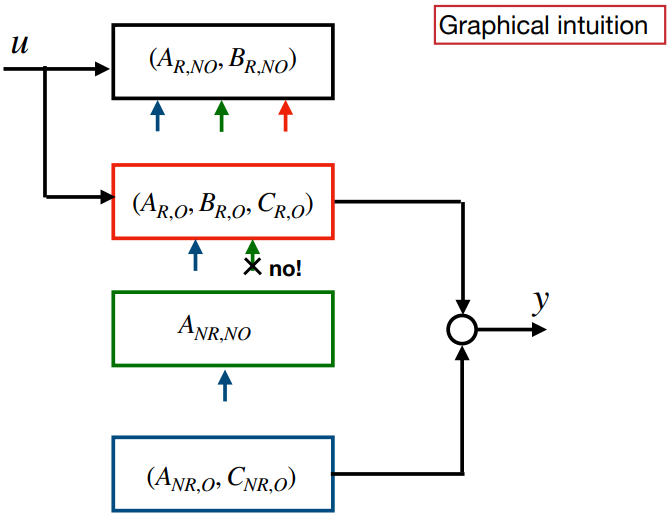
\includegraphics[width=0.8\linewidth]{images/Ult_Kalman}
\end{figure*}

Connections fromt the top to the bottom would all violate non-reachability/non-observability properties of the subsystems, while most connections from the bottom to the top are permissible.

\begin{theorem}
    Given $(A,B,C)$ The following T:
    \[
        T^{-1}:=\begin{bmatrix}
            \mathcal{R}^+ \cap \mathcal{E}_{NO} & \mathcal{R}^+ \cap \mathcal{E}^+ & \mathcal{R}^+_{NR} \cap \mathcal{E}^+_{NO} & \mathcal{R}^+_{NR} \cap \mathcal{E}^+ 
        \end{bmatrix}
    \]
    makes the system in the following Kalman form:
    \begin{gather*}
        \tilde{A} = TAT^{-1} := \begin{pmatrix}
            A_{R,NO} & A_{R,NO}' & A_{R,NO}'' & A_{R,NO}'''\\
            0 & A_{R,O} & 0 & A_{R,O}'\\
            0 & 0 & A_{NR,NO} & A_{NR,NO}'\\
            0 & 0 & 0 & A_{NR,O}
        \end{pmatrix} \quad \tilde{B}=TB:= \begin{pmatrix}
            B_{R,NO}\\B_{R,O}\\0\\0
        \end{pmatrix} \\ \tilde{C} = CT^{-1}:=\begin{pmatrix}
            0 & C_{R,O} & 0 & C_{NR,O}
        \end{pmatrix}
    \end{gather*}
    where
    \begin{gather*}
        (A_{R,NO},B_{R,NO}) \text{ is completely controllable} \qquad \qquad \qquad (A_{R,O},C_{R,O}) \text{ is completely observable}\\
        \left( \begin{pmatrix}
            A_{R,NO} & A'_{R,NO}\\
            0 & A_{R,O}
        \end{pmatrix}, \begin{pmatrix}
            B_{R,NO}\\B_{R,O}
        \end{pmatrix} \right) \text{ is completely controllable} \\ \left( 
            \begin{pmatrix}
                A_{R,O} & A'_{R,O}\\
                0 & A_{NR,O}
            \end{pmatrix},\begin{pmatrix}
                C_{R,O} & C_{NR_O}
            \end{pmatrix}\right) \text{ is completely observable}
    \end{gather*}
\end{theorem}




\chapter{NL control via linearization}
\begin{flalign*}
    &\left. \begin{array}{r} 
        \dot{{x}}(t)\\[1ex]
        {}{x}(t+1)
        \end{array} \right\} 
        =f(x(t),u(t)) \qquad x(0)=x_0\\
        &y(t)=h(x(t))
\end{flalign*}

\section{set point control}
Goal: to steer the regulated output $y$ (coincident with the measured output) to a set point $y^\star=\text{const.}$ by properly controlling the system via state or output feedback

Let $(x^\star, u^\star)$ be the solution of the system inversion
\begin{observation}
    \begin{itemize}
        \item $(x^\star, u^\star)$ are the desired steady state for the state and the input
        \item they are uncertain if the system is
    \end{itemize}
\end{observation}
\subsection{Linearization}
\begin{align*}
    \dot{x}=f(x,u)=f(x^\star, u^\star)+ \eval{\frac{\partial f(x,u)}{\partial x}}{x^\star,u^\star}(x-x^\star)+ \eval{\frac{\partial f(x,u)}{\partial u}}{x^\star,u^\star} (u-u^\star) + h.o.t(\tilde{x},\tilde{u})\\
    y=h(x)=h(x^\star)+ \eval{\frac{\partial h(x)}{\partial x}}{x^\star}(x-x^\star)+h.o.t(\tilde{x})
\end{align*}

\begin{gather*}
    A=\begin{pmatrix}
        \frac{\partial f_1(x,u)}{\partial x_1} & \frac{\partial f_1(x,u)}{\partial x_2} & \cdots & \frac{\partial f_1(x,u)}{\partial x_n}\\
        \frac{\partial f_2(x,u)}{\partial x_1} & \frac{\partial f_2(x,u)}{\partial x_2} & \cdots & \frac{\partial f_2(x,u)}{\partial x_n}\\
        \vdots & \vdots & \ddots & \vdots \\
        \frac{\partial f_n(x,u)}{\partial x_1} & \frac{\partial f_n(x,u)}{\partial x_2} & \cdots & \frac{\partial f_n(x,u)}{\partial x_n}
    \end{pmatrix}_{x=x^\star,u=u^\star} \qquad \quad B=\begin{pmatrix}
        \frac{\partial f_1(x,u)}{\partial u} \\ \frac{\partial f_2(x,u)}{\partial u} \\ \vdots \\ \frac{\partial f_n(x,u)}{\partial u}
    \end{pmatrix}_{x=x^\star, u=u^\star} \quad \quad C^T=\begin{pmatrix}
        \frac{\partial h(x)}{\partial x} \\ \frac{\partial h(x)}{\partial x} \\ \vdots \\ \frac{\partial h(x)}{\partial x}
    \end{pmatrix}_{x=x^\star}
\end{gather*}

\begin{flalign*}
    &\left. \begin{array}{r} 
        \dot{{x}}(t)\\[1ex]
        {}{x}(t+1)
        \end{array} \right\} 
        =A\tilde{x}(t)+B\tilde{u}(t)+g_f(\tilde{x}(t),\tilde{u}(t)) \qquad \tilde{x}(0)=\tilde{x}_0\\
        &\tilde{y}(t)=C\tilde{x}(t)+g_h(\tilde{x}(t))
\end{flalign*}
where
\begin{flalign*}
    \tilde{x}:=x-x^\star\\
    \tilde{u}:=u-u^\star\\
    \tilde{y}:=y-y^\star\\
\end{flalign*}

\subsection{state feedback solution}
If $(A,B)$ is stabilizable we could design $u(t)$ so that $\tilde{u}(t)=K\tilde{x}(t)$ with $K$ such that $A+BK$ is Hurwitz/Schur\\

\begin{flalign*}
    &\left. \begin{array}{r} 
        \dot{\tilde{x}}(t)\\[1ex]
        {}\tilde{x}(t+1)
        \end{array} \right\} 
        =(A+BK)\tilde{x}(t)+g_f(\tilde{x}(t),K\tilde{x}(t)) \qquad \tilde{x}(0)=\tilde{x}_0\\
        &u(t)=u^\star + K(x(t)-x^\star)
\end{flalign*}

By the indirect Lyapunov theorem we know that $\tilde{x}=0$ is LAS for the nonlinear controlled system.\\
Robustness issues: \begin{itemize}
    \item $u^\star$ is uncertain
    \item $K:A_\mu B_\mu K$ Hurwitz. If the actual values $(A,B)$ are close to the nominal ones $(A_\mu,B_\mu)$ it's not a big problem
\end{itemize}
This solution is only valid in the domain of attraction, which depends on the nonlinearities of the system.
\subsection{output feedback solution}
If $(A,B)$ is stabilizable and $(A,C)$ is detectable we could design $u(t)$ so that $\tilde{u}(t)=K\hat{\tilde{x}}(t)$ with $K$ such that $A+BK$ is Hurwitz/Schur and $\hat{\tilde{x}}$ generated by an asymptotic observer in which the output injection matrix $L$ is chosen so that $A+LC$ is Hurwitz/Schur
\begin{flalign*}
    &\left. \begin{array}{r} 
        \dot{\hat{\tilde{x}}}(t)\\[1ex]
        {}\hat{\tilde{x}}(t+1)
        \end{array} \right\} 
        =(A+BK)\hat{\tilde{x}}(t)+L(C\hat{\tilde{x}}(t)-\tilde{y}(t)) \\
        &u(t)=u^\star + K\hat{\tilde{x}}(t)
\end{flalign*}

By letting $e:=\hat{\tilde{x}}-\tilde{x}$, it turns out that the closed-loop is (C-T case)
\[
    \begin{pmatrix}
        \dot{\tilde{x}}\\\dot{e}
    \end{pmatrix}=\begin{pmatrix}
        A+BK & BK\\
        0 & A+LC
    \end{pmatrix}\begin{pmatrix}
        \tilde{x}\\e
    \end{pmatrix}+\begin{pmatrix}
        g_f(\tilde{x},K\tilde{x}+Ke) \\ -g_f(\tilde{x},K\tilde{x}+Ke)-Lg_h(\tilde{x})
    \end{pmatrix}
\]
By the indirect Lyapunov theorem we know that $(\tilde{x},e)$ is LAS for the nonlinear controlled system\\
Same locality and robustness issues as the previous case
\subsection{Integral action}
To robustify the asymptotic performance of the controller we can add integral action by extending the system:\\
\begin{gather*}
    \dot{x}(t)=f(x(t),u(t)) \quad x(0)=x_0\\
    y(t)=h(x(t))\\
    \dot{\sigma}=\tilde{y}=h(x)-y^\star \quad \text{ bunch of p integrators}
\end{gather*}
We deal with square systems: $u,y \in \R^p$
Target equilibrium:
\begin{gather*}
    x^\star=f(x^\star,u^\star)\\
    y^\star=h(x^\star)
    \sigma^\star=\text{any}
\end{gather*}

Linearization of the system around the target equilibrium:

\begin{gather*}
    \dot{\tilde{x}}=A\tilde{x}+B\tilde{u} +g_f(\tilde{x},\tilde{u})\\
    \dot{\tilde{\sigma}}=C\tilde{x}+g_h(\tilde{x})
\end{gather*}

In compact form:

\[
    \begin{pmatrix}
        \dot{\tilde{\sigma}} \\ \dot{\tilde{x}}
    \end{pmatrix} = \begin{pmatrix}
        A & 0 \\ C & 0
    \end{pmatrix}\begin{pmatrix}
        \tilde{x} \\ \tilde{\sigma}
    \end{pmatrix}+\begin{pmatrix}
        B \\ 0
    \end{pmatrix}\tilde{u} + \begin{pmatrix}
        g_f(\tilde{x},\tilde{u}) \\ g_h(\tilde{x})
    \end{pmatrix}=\mathcal{A}\begin{pmatrix}
        \tilde{x} \\ \tilde{\sigma}
    \end{pmatrix}+\mathcal{B}\tilde{u} + \begin{pmatrix}
        g_f(\tilde{x},\tilde{u}) \\ g_h(\tilde{x})
    \end{pmatrix}
\]
if $(\mathcal{A},\mathcal{B})$ is stabiilizable then there exists a $\mathcal{K}=[K_x,K_\sigma]$ such that $\mathcal{A}+\mathcal{B}\mathcal{K}$ is Hurwitz. So, let's choose $\tilde{u}=K_x\tilde{x}+K_\sigma \tilde{\sigma}$ so that the origin $(\tilde{x},\tilde{\sigma})=(0,0)$ is LAS (robust). (Note: $K_\sigma$ is square $(p \times p)$)
\begin{result}
    if $\mathcal{K}$ is such that $\mathcal{A}+\mathcal{B}\mathcal{K}$ is Hurwitz, then necessarily $K_\sigma$ is non singular
\end{result}

we can pick $\sigma^\star=\bar{\sigma}^\star := K_\sigma^{-1}(u^\star-K_xx^\star)$

\begin{result}
    ($\mathcal{A},\mathcal{B}$) is controllable if $(A,B)$ is controllable and the following non resonance condition is fuliflled:
    \[
        rank\begin{pmatrix}
            -A & B\\
            C &  0\\
        \end{pmatrix}=n+p
    \]
\end{result}

The initial condition must lay within the domain of attraction in order for the LAS property of the system to be of any use. $\sigma(0)$ must therefore be initialized to an appropriate value inside the domain of attraction. If the uncertainties on the system are large, the chosen $\sigma(0)$ might fall outside the actual domain of attraction.

\subsection{Gain scheduling}
The idea is, in order to overcome the locality of the linearization approach, to switch between setpoints, each having their own linearized control, with overlapping domains of attraction.

Let's introduce a gain scheduling variable $\alpha$ and let $(x^\star(\alpha),u^\star(\alpha))$ be solution of\[
    \left\{ \begin{array}{l}
        0=f(x^\star(\alpha),u^\star(\alpha))\\[1ex]
        {}\alpha=h(x^\star(\alpha))
        \end{array} \right.
    \]
Following the design procedure proposed in the robust integral-based solution let
\[
    \mathcal{A}(\alpha)=\begin{pmatrix}
        A(\alpha) & 0 \\
        C(\alpha) & 0
    \end{pmatrix} \quad \mathcal{B}(\alpha)=\begin{pmatrix}
        B(\alpha) \\ 0
    \end{pmatrix} \text{ with } \mathcal{K}(\alpha)=[K_x(\alpha),K_\sigma(\alpha)] \text{ such that } \mathcal{A}(\alpha)+\mathcal{B}(\alpha)\mathcal{K}(\alpha) \text { is Hurwitz}
\]
This makes a robust controller parametrized by $\alpha$:
\begin{gather*}
    \dot{\sigma}=y-\alpha\\
    u=K_x(\alpha)x+K_\sigma(\alpha)\sigma
\end{gather*}
If $(x(0),\sigma(0))$ are sufficiently close to $(x^\star(\alpha),\bar{\sigma}^\star(\alpha))$ then $x(t)\to x^\star(\alpha)$ and $y(t) \to \alpha$. Idea: to substitute $\alpha$ with a slow varying $y^\star(t)$. We get a linear time-varying controller:
\begin{gather*}
    \dot{\sigma}=y-y^\star(t)\\
    u=K_x(y^\star(t))x+K_\sigma(y^\star(t))\sigma
\end{gather*}

\begin{result}
    $\exists \epsilon_1, \epsilon_2$ (small) positive numbers such that if $\|\dot{y}^\star(t)\|\leq\epsilon_1$ and $\forall (x_0,\sigma_0)$ such that
    \[
        \|(x_0,\sigma_0)-(x^\star(y^\star(0)),\bar{\sigma}^\star(y^\star(0)))\|\leq\epsilon_2
    \]
    then the following holds:
    \begin{itemize}
        \item The trajectories of the closed loop system are bounded
        \item $\exists c,T>0$ such that $\|y(t)-y^\star(t)\|\leq c\epsilon_1 \quad \forall t \geq T$
        \item if $\lim_{t\to\infty}\dot{y}^\star(t)=0$ then $\lim_{t\to\infty}y(t)-y^\star(t)=0$
        \end{itemize}
\end{result}

\chapter{Feedback linearization}
Problem of feedback linearization: Finding a state feedback control law $u=\alpha(x)+v$, whith $v$ an auxiliary input, and a coordinate change $z=\Phi(x)$ such that the controlled system described in the new form $\dot{z}=Az+Bv$ with $(A,B)$ completely controllable.
\section{relative degree}
\begin{definition}[Lie derivative]
    Let $f:\R^n\to\R^n$, $g:\R^n\to\R^n$, $h:\R^n\to\R$. The Lie derivative of $h(x)$ along $f(x)$ is defined as:
    \[
        L_fh(x):=\frac{dh}{dx}f(x):\R^n\to\R
    \]
    The 2nd order Lie derivative of $h(x)$ along $f(x)$ is:
    \[
        L_f^2h(x):=L_f(L_fh(x))=\frac{d\frac{dh}{dx}f(x)}{dx}f(x):\R^n\to\R
    \]
    We also define the following:
    \begin{gather*}
        L_f^kh(x):=L_fL_f^{k-1}h(x) \qquad L_f^0h(x):=h(x)\\
        L_gL_fh(x):=\frac{d\frac{dh}{dx}f(x)}{dx}g(x):R^n\to\R
    \end{gather*}
\end{definition}
\begin{observation}
    it represents the derivative of $h(x)$ along the direction of $f(x)$\\
    the operator is linear. In particular: $L_f(\alpha_1h_1(x)+\alpha_2h_2(x))=\alpha_1L_fh_1(x)+\alpha_2L_fh_2(x)$
\end{observation}

\begin{definition}[relative degree]
    The system $(f(x),g(x),h(x))$ has relative degree $r$ at $\bar{x}$ if
    \begin{itemize}
        \item $L_gL_f^kh(x)=0$ $\forall x$ in a  neighbourhood of $\bar{x}$ and $\forall k = 0,1,\dots,r-2$
        \item $L_gL_f^{r-1}h(x)\neq 0$ (and thus by continuity $L_gL_f^{r-1}h(x)\neq 0 \forall x$ in a neighbourhood of $\bar{x}$)
    \end{itemize}
\end{definition}

\begin{result}
    if $r$ exists then $r\leq n$
\end{result}
\section{Normal form}
\begin{result}
    Suppose that $(f(x),g(x),h(x))$ has relative degree $r$ at $\bar{x}$. Then
    \[
        rank \begin{pmatrix}
            \frac{dh(x)}{dx}\\\frac{dL_fh(x)}{dx}\\\vdots\\\frac{dL_f^{r-1}h(x)}{dx}
        \end{pmatrix}_{x=\bar{x}} = r
    \]
\end{result}

Similarly to what done with the Brunowsky canonical form, we can obtain a diffeomorphism by adding $n-r$ additional functions
\[
    \Phi(x)=\begin{pmatrix}
        \Phi_1(x):=\frac{dh(x)}{dx}\\\vdots\\\Phi_r(x):=\frac{dL_f^{r-1}h(x)}{dx}\\ \Phi_{r+1}(x)\\\vdots\\\Phi_n(x)
    \end{pmatrix}
\]
constructed such that $rank\eval{\frac{d\Phi(x)}{dx}}{x=\bar{x}}=n.$
Remark: it is always possible to choose $\Phi_i(x),i=r+1,\dots,n$ such that $L_g\Phi_i(x)=0$ for all $x$ in a neighbourhood of $x$\\
With this change of coordinates
\[
    z=\Phi(x)\qquad z=\begin{pmatrix}
        \xi\\\eta
    \end{pmatrix} \qquad \xi=\begin{pmatrix}
        \Phi_1(x) \\ \vdots \\ \Phi_r(x)
    \end{pmatrix} \qquad \eta=\begin{pmatrix}
        \Phi_{r+1}(x) \\ \vdots \\ \Phi_n(x)
    \end{pmatrix}
\]
we obtain
\begin{gather*}
    \dot{\xi}_i=\xi_{i+1} \quad i=1,\dots,r-1 \quad y=\xi_1\\
    \dot{\xi}_r=q(\xi,\eta)+b(\xi,\eta)u \qquad b(\xi,\eta)=L_gL_f^{r-1}h(\Phi^{-1}(z))\\
    \dot{\eta}=\varphi(\xi,\eta)
\end{gather*}

\section{Feedback linearisation}
\begin{theorem}
    The problem of feedback linearisation around a $\bar{x}$ is solvable iff there exists a $h:\R^n\to\R$ such that the system $(f(x),g(x),h(x))$ has a well defined relative degree of $n$ at $\bar{x}$
\end{theorem}
\begin{proof}[if part]
    The normal form of the system is
    \begin{gather*}
        \dot{\xi}_{i+1}=\xi_i \quad i=1,\dots,n-1\\
        \dot{\xi}_n=L_f^nh(x)+L_gL_f^{n-1}h(x)u
    \end{gather*}
\end{proof}
The feedback linearising control law is thus
\[
    u=\frac{1}{L_gL_f^{n-1}h(x)}(-L_f^nh(x)+v)
\]
The controllable $(A,B)$ is therefore
\[
    A=\begin{pmatrix}
        0 & 1 & 0 & \cdots & 0\\
        0 & 0 & 1 & \cdots & 0\\
        \vdots & \vdots & \vdots & \ddots & \vdots\\
        0 & 0 & 0 & \cdots & 1\\
        0 & 0 & 0 & \cdots & 0
    \end{pmatrix} \qquad B=\begin{pmatrix}
        0 \\ 0 \\\vdots \\ 0 \\ 1
    \end{pmatrix}
\]

\section{Zero dynamics and minimum-phaseness}
Let's assume $\bar{x}=0$ and that $\Phi(\cdot)$ is chosen so that $\Phi(0)=0$ $(\bar{z}=0)$\\
If the system $(f(x),g(x),h(x))$ has a well defined relative degree $r\leq n $ (at $\bar{x}=0$) then the zero dynamics of the system are $\dot{\eta}=\varphi(\eta,0)$ (dimension $n-r$)\\
The terminology "zero dynamics" is justified by the fact that those are dynamics of the system compatible with $y(t)=0$  $\forall t$ and for the fact that for linear systems the eigenvalues that govern those dynamics coincide with the zeros of the transfer function

\begin{definition}[minimum-phase system]
    The system $(f(x),g(x),h(x))$ is said to be minimum-phase if $\bar{\eta}=0$ is LAS for the zero dynamics $\dot{\eta}=\varphi(\eta,0)$
\end{definition}
\begin{definition}[strongly minimum-phase system]
    The system $(f(x),g(x),h(x))$ is said to be strongly minimum-phase at $\bar{x}$ if the zero dynamics $\dot{\eta}=\varphi(\eta,0)$ are ISS wrt the input $\xi$
\end{definition}


\end{document}
